\documentclass[a4paper,12pt,oneside,openright]{memoir}
\chapterstyle{veelo}

%\documentclass[draft,final]{vutinfth} % Remove option 'final' to obtain debug information.

\usepackage{TUINFDA}
\usepackage{url}
\usepackage[colorlinks=true,urlcolor=blue]{hyperref}					% links in pdf
\usepackage{graphicx}            			% Figures
\usepackage{verbatim}            			% Code-Environment
\usepackage{listings}
\usepackage{graphicx}
\usepackage{caption}
\usepackage{subfig}
\usepackage{float}
\usepackage{amsmath}


% hglanzer: problem workstation@labor <--> laptop
%\usepackage[lined,linesnumbered,algochapter]{algorithm2e} % Algorithm-Environment
\usepackage[lined,linesnumbered,algochapter,norelsize]{algorithm2e} % Algorithm-Environment


\usepackage{pgf}					
\usepackage{tikz}					% tikz graphics
\usetikzlibrary{arrows,automata}
\usepackage[toc]{glossaries}

\makeglossary
\loadglsentries{acronyms}

\usepackage[backend=bibtex, sorting=none]{biblatex}
\addbibresource{references.bib}

%%%%%%%%%%%%%%%%%%%%%%%%%%%%%%%%%%%%%%%%%%%%%%%%%%%%%%%%%%%%%%%%%%%%%%%%%%%%%%%%%

\thesistitle{Highly available KNX networks}
%\thesissubtitle{Building a secure and dependable Layer} % optional
\thesisdate{14.8.2015}

% all titles and designations have to be gender-related!
\thesisdegree{Diplom-Ingenieur}{Diplom-Ingenieur}
\thesiscurriculum{Technische Informatik}{Computer Engineering} % your study
\thesisverfassung{Verfasser} % Verfasser
\thesisauthor{B.Sc. Harald Glanzer} % your name
\thesisauthoraddress{Hardtgasse 25 / 12A, 1190 Wien} % your address
\thesismatrikelno{0727156} % your registration number

\thesisbetreins{Ao.Univ-Prof. DI Dr. Wolfgang Kastner}
\thesisbetrzwei{DI Dr. Lukas Krammer}
%\thesisbetrdrei{Dr. Vorname Familienname} % optional

% define page numbering styles
\makepagestyle{numberCorner}
\makeevenfoot{numberCorner}{\thepage}{}{}
\makeoddfoot{numberCorner}{}{}{\thepage}

% define custom macros for specific formats or names
\newcommand{\uml}[1]{\texttt{#1}}
\newcommand{\cd}{\textsf{Class Diagram}}

% for shell command snippets
\newcommand{\shellcmd}[1]{\\\indent\indent\texttt{\footnotesize\# #1}\\}

% for shell command snippets with multiple lines
\lstdefinestyle{BashInputStyle}{
  language=bash,
  basicstyle=\small\sffamily,
  numbers=left,
  numberstyle=\tiny,
  numbersep=3pt,
  %frame=tb,
  columns=fullflexible,
  backgroundcolor=\color{yellow!20},
  linewidth=0.9\linewidth,
  xleftmargin=0.1\linewidth,
  breaklines=true,
  showstringspaces=false,
  captionpos=b
}

\lstdefinestyle{Cstyle}{
  language=C,
  basicstyle=\small\sffamily,
  numbers=left,
  numberstyle=\tiny,
  numbersep=3pt,
  %frame=tp,			% top bottom frame
  columns=fullflexible,
  backgroundcolor=\color{yellow!20},
  linewidth=0.95\linewidth,
  xleftmargin=0.1\linewidth,
  breaklines=true,
  keepspaces=true,
  captionpos=b,
  showstringspaces=false
}

\begin{document}

\captionnamefont{\bfseries}

%%%%%%%%%%%%%%%%%%%%%%%%%%%%%%%%%%%%%%%%%
%%%   FRONTMATTER    %%%%%%%%%%%%%%%%%%%%
%%%%%%%%%%%%%%%%%%%%%%%%%%%%%%%%%%%%%%%%%
\frontmatter
\pagenumbering{roman}

%%%%%%%%%%%%%%%%%%%%%%%%%%%%%%%%%%%%%%%%%
%%%   TITLEPAGES    %%%%%%%%%%%%%%%%%%%%%
%%%%%%%%%%%%%%%%%%%%%%%%%%%%%%%%%%%%%%%%%

% the german title page is required as first page
\include{titlepage}

% an english translation may follow
\include{titlepage_en} % optional

%%%%%%%%%%%%%%%%%%%%%%%%%%%%%%%%%%%%%%%%%
%%%   ERKLAERUNG DER SELBSTAENDIGKEIT   %
%%%%%%%%%%%%%%%%%%%%%%%%%%%%%%%%%%%%%%%%%
\cleardoublepage
\selectlanguage{ngerman}
\input{chapters/erklaerung}
\selectlanguage{english}

%%%%%%%%%%%%%%%%%%%%%%%%%%%%%%%%%%%%%%%%%
%%%   ACKNOWLEDGEMENTS    %%%%%%%%%%%%%%%
%%%%%%%%%%%%%%%%%%%%%%%%%%%%%%%%%%%%%%%%%

% optional acknowledgements may be included in german or in english
\selectlanguage{ngerman}
\chapter*{Danksagung}

An dieser Stelle - zum Abschluss des Studiums durch diese Arbeit - sollen alle jene dankend erwähnt werden, welche dies ermöglicht und mitgeholfen haben.
\\
\\
Der allererste Platz gebührt hier natürlich meinem engsten Familienkreis. Meine Eltern Christine und Hans haben mir die Überzeugung mitgegeben, dass eine solide Ausbildung ein
sehr hohes Gut und eine hervorragende Investition in die Zukunft ist, und meine Schwestern Michaela und Christina haben mir das immer vorgelebt.
\\
\\
Meine Freundin Sonja war es, die zu oft, v.a. gegen Ende meines Studiums, negative Schwingungen abbekommen und mich trotzdem immer voll und ganz unterstützt hat.
\\
\\
Bei Ao.Univ-Prof. DI Dr. Wolfgang Kastner Wolfgang Kastner und DI Dr. Lukas Krammer möchte ich mich bedanken dass Sie mir ermöglicht haben, die Diplomarbeit unter ihren Fittichen
zu schreiben. Ganz allgemein war das Institute of Computer Aided Automation, mit allen die dazugehören, ein sehr angenehmer Arbeitsplatz. Danke dafür!
\\
\\
Danke sagen möchte ich auch dem österreichischen Staat, welcher mit hohem Einsatz ein offenes Universitätsnetz betreibt und mir mittels finanzieller Unterstützung
einen zwanglosen Umstieg vom Berufs- ins Studentenleben ermöglicht hat. 		% optional
\selectlanguage{english}
%\input{chapters/acknowledgements}	% optional

%%%%%%%%%%%%%%%%%%%%%%%%%%%%%%%%%%%%%%%%%
%%%   ABSTARCT    %%%%%%%%%%%%%%%%%%%%%%%
%%%%%%%%%%%%%%%%%%%%%%%%%%%%%%%%%%%%%%%%%

\chapter*{Abstract}
\gls{hbas} denominates systems for controlling building applications summarized under the term \gls{hvac}. Parameters can thus be controlled in a centralized manner, 
promising lower maintenance and energy costs and higher comfort. Security aspects were often neglected because the used hardware platforms lacked the needed processing power
and malicious attacks against such systems ignored.
\\
Nevertheless, corporate buildings as well as private homes contain a great variety of additional applications, for example access controls, burglar alarm or fire detection systems.
This group of applications makes much greater demands regarding the underlying technical system. Obviously, access must be only granted to authenticated persons and fire detection
systems must work reliable in case of emergency. 
\\
The different requirements lead to a separation of critical and uncritical systems, unifying them into one system would allow to further decrease maintenance costs and re-use
the existing infrastructure for both fields of application 
\\
\\
Therefore, this thesis proposes a extension to \gls{knx} which is suitable for critical environments. For this purpose it is necessary to detect and guard against malicious attacks
as well as to cope with randomly occurring hardware faults. 


DErsteres ermöglicht der Einsatz von Kryptographie,
zweiteres kann mittels Redundanz bewerkstelligt werden. Beide Begriffe sowie \gls{knx} selbst werden ausführlich erläutert, gefolgt von dem erarbeitetem Lösungsvorschlag.
Der Ansatz unterteilt eine \gls{knx}-Installation in einen ungesicherten und einen gesicherten Teil. Letzterer ist geschützt gegen böswillige Angriffe und ausserdem doppelt ausgeführt,
womit ein teilweiser Ausfall kompensiert werden kann. Abschliessend wird der implementierte Prototyp erläutert. 
\cleardoublepage
\selectlanguage{ngerman}
\chapter*{Kurzfassung}
\gls{hga} befasst sich mit Systemen zur Steuerung bzw. Regelung von Gebäudeanwendungen, wie Heizungen, Klimaanlagen oder Beleuchtungssystemen. Raumparameter
können so zentral gesteuert werden, wodurch sowohl der Verwaltungsaufwand als auch den Energieverbrauch gesenkt und der Komfort erhöht werden kann. 
Sicherheitstechnische Überlegungen spielten traditionellerweise eine untergeordnete Rolle.
Einerseits standen die Ressourcen auf den verwendeten Plattformen oft nicht zur Verfügung, andererseits wurden die Auswirkungen eines böswilligen Eingriffes in das System vernachlässigt.
%Zusätzlich ist z.B. die optimale Regelung der Raumtemperatur in einem
%Bürogebäude wichtig für den Komfort der darin arbeitenden Menschen, was sich auch auf die Produktivität auswirken kann.
\\
Firmengebäude wie Privatgebäude beherbergen jedoch eine viel grössere Anzahl an Applikationen, man denke hier an Zugangskontrollen, 
Alarmanlagen oder Brandlöschsysteme. Diese Gruppe von Anwendungen stellt höhere Anforderungen an das zugrunde liegende technische System:
Türe dürfen nur von authorisierten Personen geöffnet werden, Alarmanlagen dürfen sich nicht einfach von Einbrechern deaktivieren lassen, und Brandmeldesysteme müssen im
Extremfall mit einem hohen Grad an Zuverlässigkeit funktionieren. 
\\
Diese unterschiedlichen Anforderungen führten zu einem Auseinanderwachsen der vorhandenen Systeme. Das Zusammenführen 
von kritischen und unkritischen Systemen würde einerseits den Verwaltungsaufwand weiter senken und zusätzlich erlauben, die vorhandene Infrakstruktur, z.B. die Verkabelung,
für beide Anwendungsgebiete zu verwenden.
\\
\\
Diese Arbeit beschäftigt sich deshalb mit einer Erweiterung des \gls{knx} Standards für die \gls{hga}, die auch in kritischen Umgebungen eingesetzt werden kann.
Dazu ist es einerseits nötig, böswillige Angriffe zu erkennen und zu verhindern als auch technische Defekte abfedern zu können. Ersteres ermöglicht der Einsatz von Kryptographie,
zweiteres kann mittels Redundanz bewerkstelligt werden. Beide Begriffe, sowie \gls{knx} selbst, werden ausführlich erläutert, gefolgt von dem erarbeitetem Lösungsvorschlag.
Der Ansatz unterteilt eine \gls{knx}-Installation in einen ungesicherten und einen gesicherten Teil. Letzterer ist geschützt gegen böswillige Angriffe und ausserdem doppelt ausgeführt,
womit ein teilweiser Ausfall kompensiert werden kann. Der Aufbau der vorgeschlagenen Lösung wird beschrieben und abschliessend der implementierte Prototyp erläutert. 

\selectlanguage{english}

%%%%%%%%%%%%%%%%%%%%%%%%%%%%%%%%%%%%%%%%%
%%%   CONTENTS    %%%%%%%%%%%%%%%%%%%%%%%
%%%%%%%%%%%%%%%%%%%%%%%%%%%%%%%%%%%%%%%%%
% uncomment to set document language to german (results in "Inhaltsverzeichnis", "Kapitel", "Abbildung", etc. instead of "Contents", "Chapter", and "Figure"), otherwise the document's language is english
%\selectlanguage{ngerman}

\setcounter{tocdepth}{1}

\cleardoublepage
\pagestyle{numberCorner}
\tableofcontents*

%%%%%%%%%%%%%%%%%%%%%%%%%%%%%%%%%%%%%%%%%
%%%   MAINMATTER    %%%%%%%%%%%%%%%%%%%%%
%%%%%%%%%%%%%%%%%%%%%%%%%%%%%%%%%%%%%%%%%

\mainmatter
\pagenumbering{arabic}
\pagestyle{numberCorner}

%%%%%%%%%%%%%%%%%%%%%%%%%%%%%%%%%%%%%%%%%
\chapter{Introduction}
\label{ch:intro}
\section{Structure of the Master's Thesis}

\subsection{Motivation}

\subsection{Problem Statement}

\subsection{Aim of the work}

\subsection{Structure of the work}





%%%%%%%%%%%%%%%%%%%%%%%%%%%%%%%%%%%%%%%%%

%%%%%%%%%%%%%%%%%%%%%%%%%%%%%%%%%%%%%%%%%
\chapter{Prerequisites}
\label{ch:prerequisites}
\input{chapters/chap2Basics}
\input{chapters/chap2Cryptography}
%%%%%%%%%%%%%%%%%%%%%%%%%%%%%%%%%%%%%%%%%


%%%%%%%%%%%%%%%%%%%%%%%%%%%%%%%%%%%%%%%%%
\chapter{Availability}
\label{ch:availability}

\section{Introduction}\label{sec:availability}

Availability measures the delivery of correct service as a fraction of the time that the system is ready to provide a service. 
\\
%A system is an entity that interacts with other entities, which constitute the environment of the system and
%can be other systems, humans or the physical world \cite{1335465}. Fundamental properties of communication systems
%are \textit{functionality, performance, security and dependability}. 
The services provided by the system through its service interface to the user(s) 
is described by the functional specification. Whenever the provided service
deviates from correct service a system failure, called \textit{outage} or \textit{downtime}\footnote{in contrast, \textit{uptime} does not guarantee correct
service - for example, a server can be 'up' but unreachable} occurs. A failure is defined to be caused originally by a fault inside the system, which may be 
dormant. Under special conditions, the fault \textit{may} become apparent and lead to an error. Faults can be categorized into random and systematic faults:
random faults are unpredictable and concern hardware: for example, because of aging, a memory cell can be damaged, but the fault may be hidden because the cell
is not used. Software and design faults belong to systematic faults. Similar to the damaged memory cell, a software bug may only 
trigger an error under special inputs. In both cases, the error then causes a deviation from the required operation of the system or a subsystem. Finally, the 
error can cause a failure if the system fails to provide the correct service:
\begin{align*}
 fault \rightarrow error \rightarrow failure
\end{align*}
Availability is measured subjectively from the system user's point of view.
While an optimal system may have availability of 1, this value is only of theoretical value because random faults can not be ruled out. Therefore,
system failures are inevitable, and availability is often given in \textit{x-9s}\footnote{read 'one-nine', 'two-nines', ...} notation, denoting the 
number of nines in the time fraction the system delivers correct service, as shown in table \ref{table:x-9}.
The availability may be asserted by the provider of the system to the customer by an
\gls{sla} - if the \gls{sla} is violated, the provider may be fined.
\begin{figure}
    \centering
    \includegraphics[width=1\textwidth]{figures/availability.eps}
    \caption{Relationship between MTTF and MTTR}
  %  \caption{Relationship between \gls{mttf} and \gls{mttr}}

    \label{fig:relmttfmttr}
\end{figure}
\begin{center}
\begin{tabular}{ c | c c  }
 \label{table:x-9}
  x & $P_{availability}$ & failure duration per year \\ \hline
  1 & 90,0000    & ~ 36 days \\
  2 & 99,0000    & ~ 3,5 days  \\
  3 & 99,9000    & ~ 9 hours \\
  4 & 99,9900    & ~ 1 hour \\
  5 & 99,9990    & ~ 5 minutes \\
  6 & 99,9999    & ~ 31 seconds \\ 
  
\end{tabular}
\end{center}
For a system with 6-9 availability, this would mean that the system provider assures that the system will be unavailable not more than about 31 seconds over a
whole year.
\\
\\
Availability is important simply because unavailable systems cause costs. Because of the relation of availability to reliability and the maintainability
of the system, as shown in Equation \ref{EQUavailability} and Figure \ref{fig:relmttfmttr}, two options to improve availability exist: either increasing
the \gls{mttf} (i.e. increasing reliability) or decreasing \gls{mttr}.
%An informal definition of a dependable system is a system which delivers a service that can be justifiable trusted. More formally,
%dependability consists of the following attributes:
%\textit{Availability}, which means that the system is ready for correct service, \textit{reliability}, the continuity of correct service,
%\textit{safety}, i.e. the avoidance of catastrophic consequences \textit{integrity}, s.t. the system cannot be modified in an unwanted manner
%and \textit{maintainability}, so that the system can be repaired in the case of a failure.
%In case of a secure system, another important property is \textit{confidentiality}, which means that no information is disclosed to unauthorized 
%entities.
\begin{align}\label{EQUavailability}
 P_{Availability} = \frac{t_{correct\ service}}{t_{total}} =  \frac{{\gls{mttf}}}{\gls{mttf}+\gls{mttr}}
\end{align}
Reliability measures the probability that the service will work as expected until time $t$:
\begin{align}\label{expFailLaw}
 R(t) = e^{-\lambda(t-t_0)}
\end{align}
\ref{expFailLaw} is known as the \textit{exponential failure law}, $\lambda$ denotes the failures per hour, its inverse $\frac{1}{\lambda}$ is
called \gls{mttf}. Reliability can also be expressed in terms of \textit{un}reliability, denoted $Q(t)$:
\begin{align}
 Q(t) = 1 - R(t)
\end{align}
Maintainability measures the time that is needed to repair a system, with $\mu$ denoting the repair rate and $\frac{1}{\mu}$ called \gls{mttr}.
\\
\\
Every system will most likely consist of different and distinct components, each with its own reliability and failure rates. The final system
will possess an overall reliability, determining its availability. To model the resulting system, the components will be put together in a mixture of
serial and parallel systems.
\begin{figure}
    \centering
    \includegraphics[width=0.8\textwidth]{figures/seriesSystem.eps}
    \caption{Model of a series system}
    \label{fig:serSys}
\end{figure}
For example, if all $i$ components, ranging from $1$ to $N$, are necessary to work correctly for the overall system to deliver correct service, this can be modeled as
a series system, see Figure \ref{fig:serSys}. This does not mean that the components are necessarily connected in a serial way, it just stresses that failure
of one single components breaks the whole system. System's reliability then equals the product of all component's reliabilities:
\begin{align}
R_{system}(t) = \prod_{i=1}^{N} R_{i}(t) 
\end{align}
In contrast, a system containing redundant components, failure of one such component must not produce an outage of the overall system. This can be modeled as
a parallel system \ref{fig:parallelSys}. Here, the overall reliability can be calculated as given in \ref{parallelSysEqu}.
\begin{figure}
    \centering
    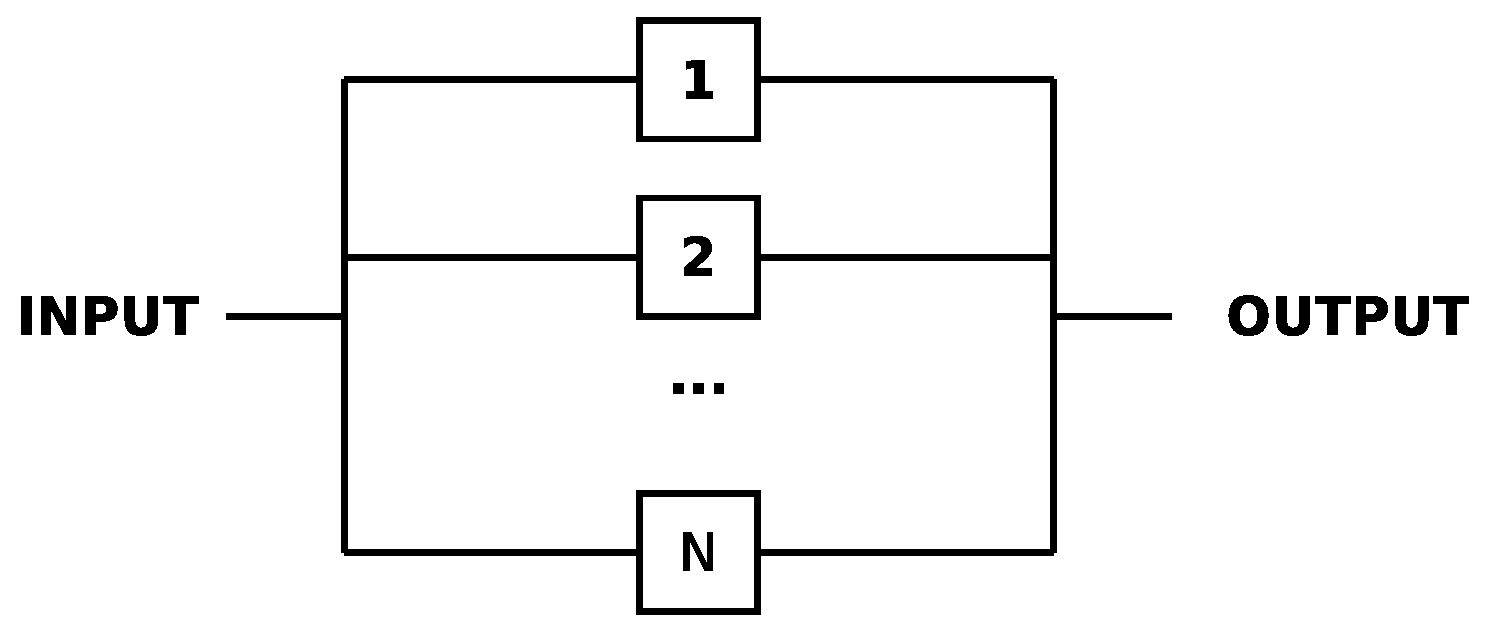
\includegraphics[width=0.8\textwidth]{figures/parallelSys.eps}
    \caption{Model of a parallel system}
    \label{fig:parallelSys}
\end{figure}

\begin{align}\label{parallelSysEqu}
 R(t)_{system} = 1 - \prod_{i=1}^{N} 1- R_{i}(t) = 1 - \prod_{i=1}^{N} Q_{i}(t)
\end{align}
Mixed systems, containing paralell and series system, can be calculated by iteratively condensing serial- or parallel subsystems into single components,
as shown in Figure \ref{fig:mixedSys}.
\begin{figure}
    \centering
    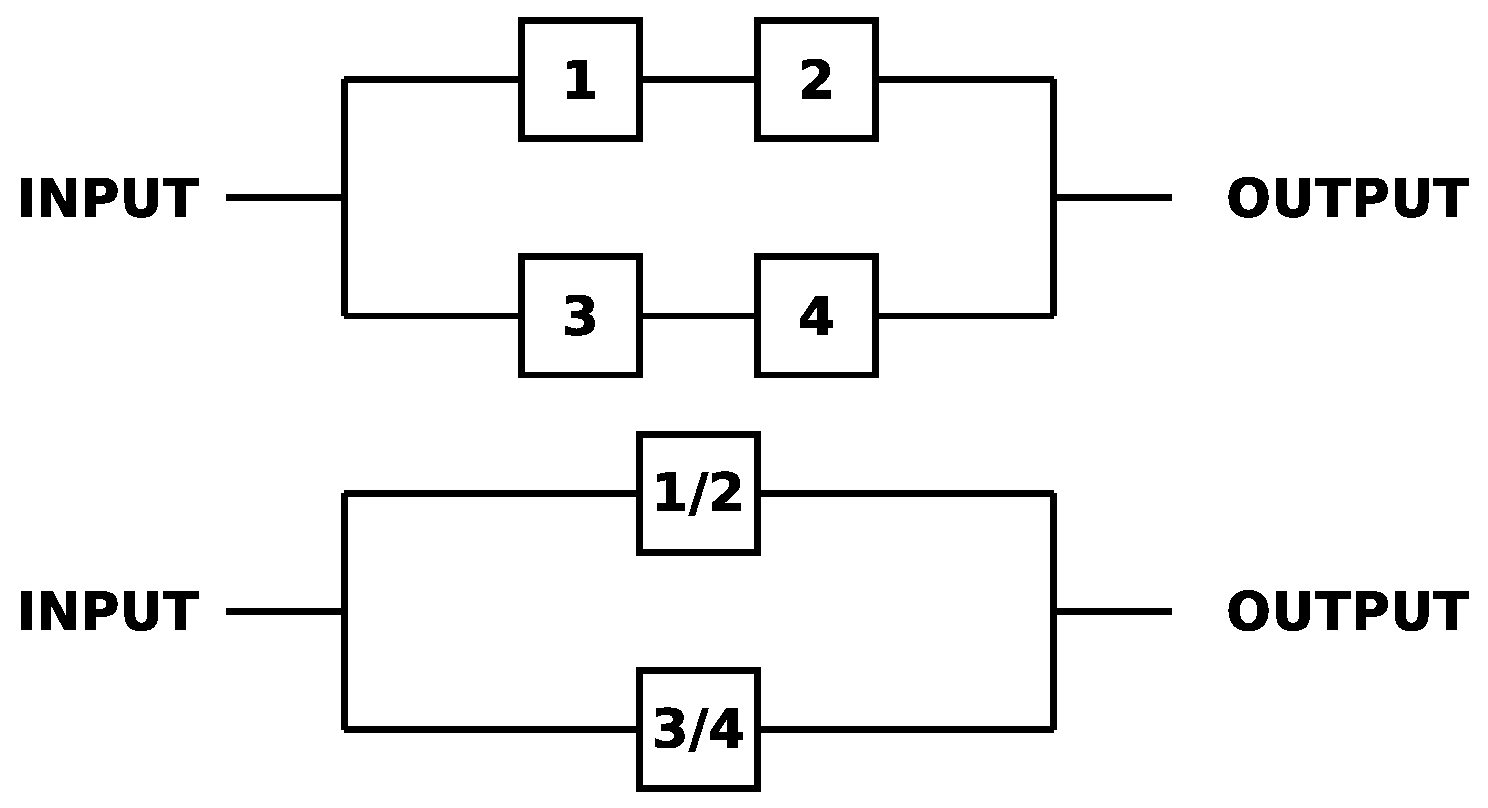
\includegraphics[width=0.8\textwidth]{figures/mixedSys.eps}
    \caption{Condensing a mixed system}
    \label{fig:mixedSys}
\end{figure}
\\
\\
\gls{ha} characterizes a system that is designed in a way to avoid outages, or in case of a failure that can be repaired in shortest possible time. 
The level of the needed availability depends on the environment of the system and must be weighted against the additional costs, introduced by improving availability.
Therefore, no hard definition for \gls{ha} can be given - it is a design goal and depends on the context. Availability requirements will most certainly be higher
for systems in safety-critical requirements. A safety-critical system must not fail, otherwise endangering human lives or 
causing substantial economic loss or environmental damage \cite{1007998}.
On the other side, systems that will produce only minor costs when not operating correctly
will probably have to meet less stringent availability levels.
\\
For example, our society heavily depends on electric power supply, an outage
is nearly unacceptable. On the other side, it is impossible to guarantee 100\% availability, so \textit{if} a power outage occurs, the system must be fixed as soon as
possible to restore correct service, otherwise risking human lives. On the contrary, a booking system will obviously result in financial losses for the company 
if not working, but no more serious consequences are to be assumed.
\\
\\
This work's focus lies on security-critical systems, increasing availability of KNX networks, but restricting its
deployment to environments without safety-critical needs. Thus, safety criticality is neglected here because of its most stringent demands, as needed in
avionics or weapons systems.
The difference between safety-critical and security-critical systems can be given as follows \cite{5784222}: safety means that software must not be harm the 
world (i.e. containment), while security means that the world must not harm software (i.e. protection).

\section{Failure Avoidance}

Different strategies exist to handle faults, thus trying to avoid that a fault propagates through the system and finally leads to a system failure.
These strategies are introduced in the next section.

\subsection{Fault Removal}
Fault removal tries to identify faults by testing the system before its deployment. 
\\
Therefore, the system is exposed to test cases, which ideally would cover all possible internal states. Whenever a failure occurs, the erroneous state is identified, the
underlying fault is removed and a new testing cycle begins.
\\
A problem about this approach is the huge test space that for even simple systems would be required to iterate through. Therefore, the method suffers from the very
fundamental dilemma that testing never can proof that a system is fault free.
\subsection{Fault Avoidance}
Fault avoidance aims at producing a system which is fault-free
per design and is applied at the design stage of the system. Despite the methods for achieving fault avoidance can be applied in the domain of sofware and hardware,
they can not guard against transient hardware faults occurring after the system is deployed.
\\
Fault avoidance is based on two distinct processing steps: validation and verification. Validation is used to to show that the specification, which is
the basis of system implementation, matches the real world within reasonable borders. This is necessary because every human built system uses an abstraction
of the real world, thus simplifying the model.
\\
In contrast, verification assures that the system indeed matches the specification. In other words, validation tries to answer if the correct system was built,
while verification is concerned about to build the system correctly.
\\
\\
Formal methods can be be utilized for verification if the system model is available in a formal language. The formal properties of the specification can then be 
checked automatically against a finite-state model of the system, a method called \textit{model checking}.
\\
While automatic validation can proof that the resulting system is correct in regard to the specification, a big problem here is to obtain the formal properties
out of an informal specification.
\\
\\
\\
Obviously, both fault removal as well as fault avoidance cannot handle deliberately introduced faults, caused by an active adversary.
Additionally, they cannot deal with hardware errors -  therefore it is argued that fault tolerance is the only practical way to guarantee availability
in a hostile environment (i.e. an environment where active attackers are assumed to exist and therefore \gls{dos} attacks cannot be ruled out), as well as to
protect against random hardware errors.
\\
Consequently, the proposed solution will be based on fault tolerance to achieve \gls{ha}, which will be examined more detailed.
 
\subsection{Fault tolerance}
Fault tolerance tries to ensure correct service despite the occurrence of faults and is achieved through error detection and subsequent system recovery.
To enable error detection, redundancy is added to a system and thereby the 
system's complexity is increased. This can be achieved both in the domain of hardware and software. 
\\
The basis of the design of fault tolerant systems is the definition of a \textit{fault hypothesis}, stating which faults must be tolerable by the system, thus
dividing the fault state into normal faults and rare faults (i.e. faults not covered by the fault hypothesis). Normal faults can be corrected by the fault-tolerance
mechanism. 

\subsubsection{Fail-silent fault tolerance}
Fault tolerance can be achieved based on \textit{fail-silent} components. A fail-silent component
either works correctly, i.e. outputs correct values, or does not output any values at all \cite{544479}. By duplicating such a module and comparing the
outputs, fault tolerance can be achieved by cutting off the faulty module from the system.
\\
This method is used for example for \gls{raid} based date storage \footnote{although the logic distributing
the data chunks to different devices can be built in hardware or in software, i.e. the operating system, \gls{raid} always relies on redundant disks}.
For \gls{raid} level 1, all data to be stored is duplicated to two independent disks. In case a hardware failure of one drive is detected, the data can be accessed
from the second drive. This method does obviously not work if both drives seem operable, but one drive outputs bogus data, i.e. it is not acting fail-silent.
To handle this situation, higher redundancy levels are needed, as implemented for example in \gls{tmr}. 

\subsubsection{\gls{tmr}}
A \gls{tmr} system, see Figure \ref{fig:tmr}, is composed out of 3 modules or \textit{black boxes}, all performing the same task,	
and one \textit{majoriy organ} $V$, as proposed by Von Neumann \cite{vN56}. The latter element
is also called \textit{voter} because out of its 3 inputs, it chooses the 'correct' output based on majority voting. As long as at least 2 black boxes do not
fail, the system can provide correct service. If it is assumed that the voting element has perfect reliability = 1 and all black boxes $M$ are independent from
each other and have reliability $R_M$, the overall, time-invariant system's reliability is given in \ref{tmrEq} \cite{Lyons:1962:UTR:1661979.1661984} and plotted in graph \ref{fig:tmrGrp}
\begin{align}\label{tmrEq}
 R_{system} = {R_M}^3 + 3{R_M}^2(1-R_M) = 3{R_M}^2 - 2{R_M}^3
\end{align}
\begin{figure}
    \centering
    \includegraphics[width=0.8\textwidth]{figures/tmr.eps}
    \caption{Non-redundant operation vs. \gls{tmr}}
    \label{fig:tmr}
\end{figure}
\begin{figure}
    \centering
    \includegraphics[width=0.8\textwidth]{figures/tmrGraph.eps}
    \caption{Reliability of resulting system}
    \label{fig:tmrGrp}
\end{figure}
It can be seen that if $R_M \leq 0.5$, overall reliability even worses, while for components reliabilities nearly being unit, very high system reliability can
be achieved.
\\
\\
The concept of \gls{tmr} can be generalized to $n$ devices performing
the same operation. In most cases $n$ will be odd, so failure of at least $\frac{n-1}{2}$ modules can be tolerated.

\section{Fault Tolerant Technologies}
In the next sections, communication protocols based on ethernet, satisfying the needs of industrial communication networks, are examined. Beside the need for high availability,
industrial production lines
are sensitive against network disruptions. While, depending on the application domain short interruptions in the range of milliseconds to seconds may be
tolerable, longer outages will force emergency stops or even cause damage.

\subsection{Network redundancy}

Communication networks can be modeled as graphs. A graph, as shown in Figure \ref{fig:graph}, is an ordered pair $G=(V,E)$, with $V$ being the set of vertices and $E$
the set of edges, connecting the vertices. For a weighted graph, every edge is associated to a \textit{cost}. 
\\
A \textit{closed walk} or \textit{cycle} exists if a path from one vertex to itself exists, resulting in multiple paths from one node to others.
Such a network posses intrinsic redundancy, a fact that can be exploited to gain fault tolerant systems.
\\
If the graph is undirected, every line determines a bidirectional communication link. 
\\
A spanning tree of graph $G$ is a subgraph $T$, possessing all vertices $V$ but only a subset of the edges $E' \subseteq E$ s.t. all vertices are reachable,
but no loops exists. In the case of a weighted graph, the weight of the spanning tree is the sum of all existing edges.
\begin{figure}[H]
\centering
 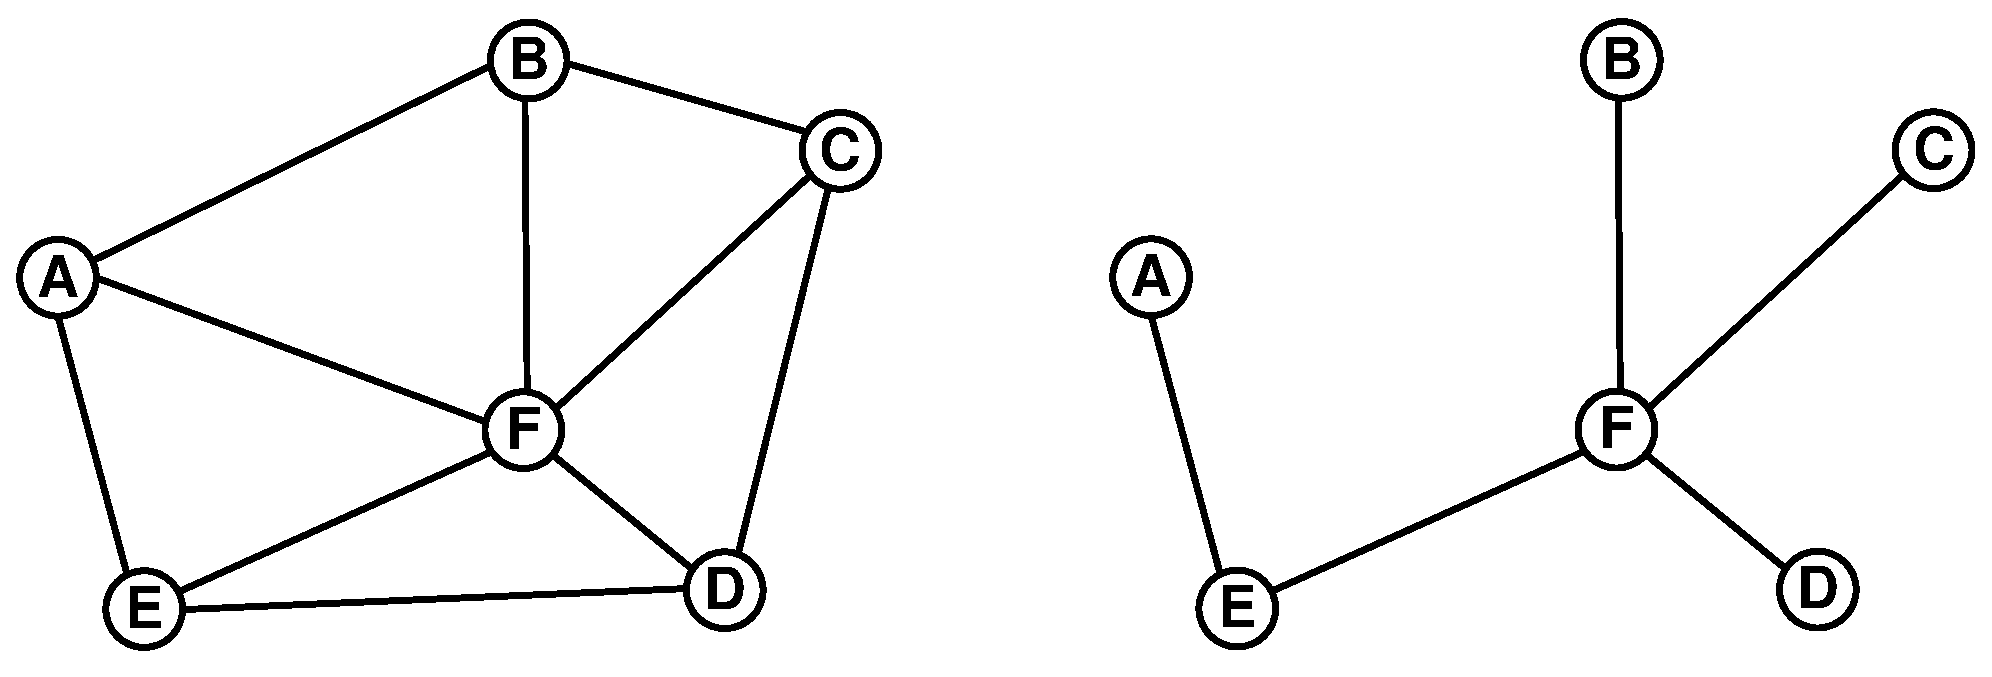
\includegraphics[width=0.8\linewidth]{figures/graph.eps}
 \caption{Undirected graph, spanning tree of the graph}
\label{fig:graph}
\end{figure}

\subsubsection{\gls{stp}}
The widely used \gls{ieee} 802.3 ethernet standard was not designed with high availability in mind.
Nevertheless, it already provided basic fault tolerance mechanisms based on the \gls{ieee} 802.1D \gls{stp}. 
\\
\\
In typical ethernet installations, depending on the network topology different
nodes may be reachable through different paths, i.e. physical loops may exist.
Switches, operating at \gls{osi} layer 2, are responsible for loop detection and
loop prevention and must logically disconnect such loops by blocking the corresponding ports to protect the network,
as required by the ethernet specification, because multicast or broadcast traffic, generated by one of the connected
devices, will be forwarded by all switches on all ports (except the incoming ports), thus flooding the network until no regular communication will be possible any
more.
\\
\begin{figure}[H]
 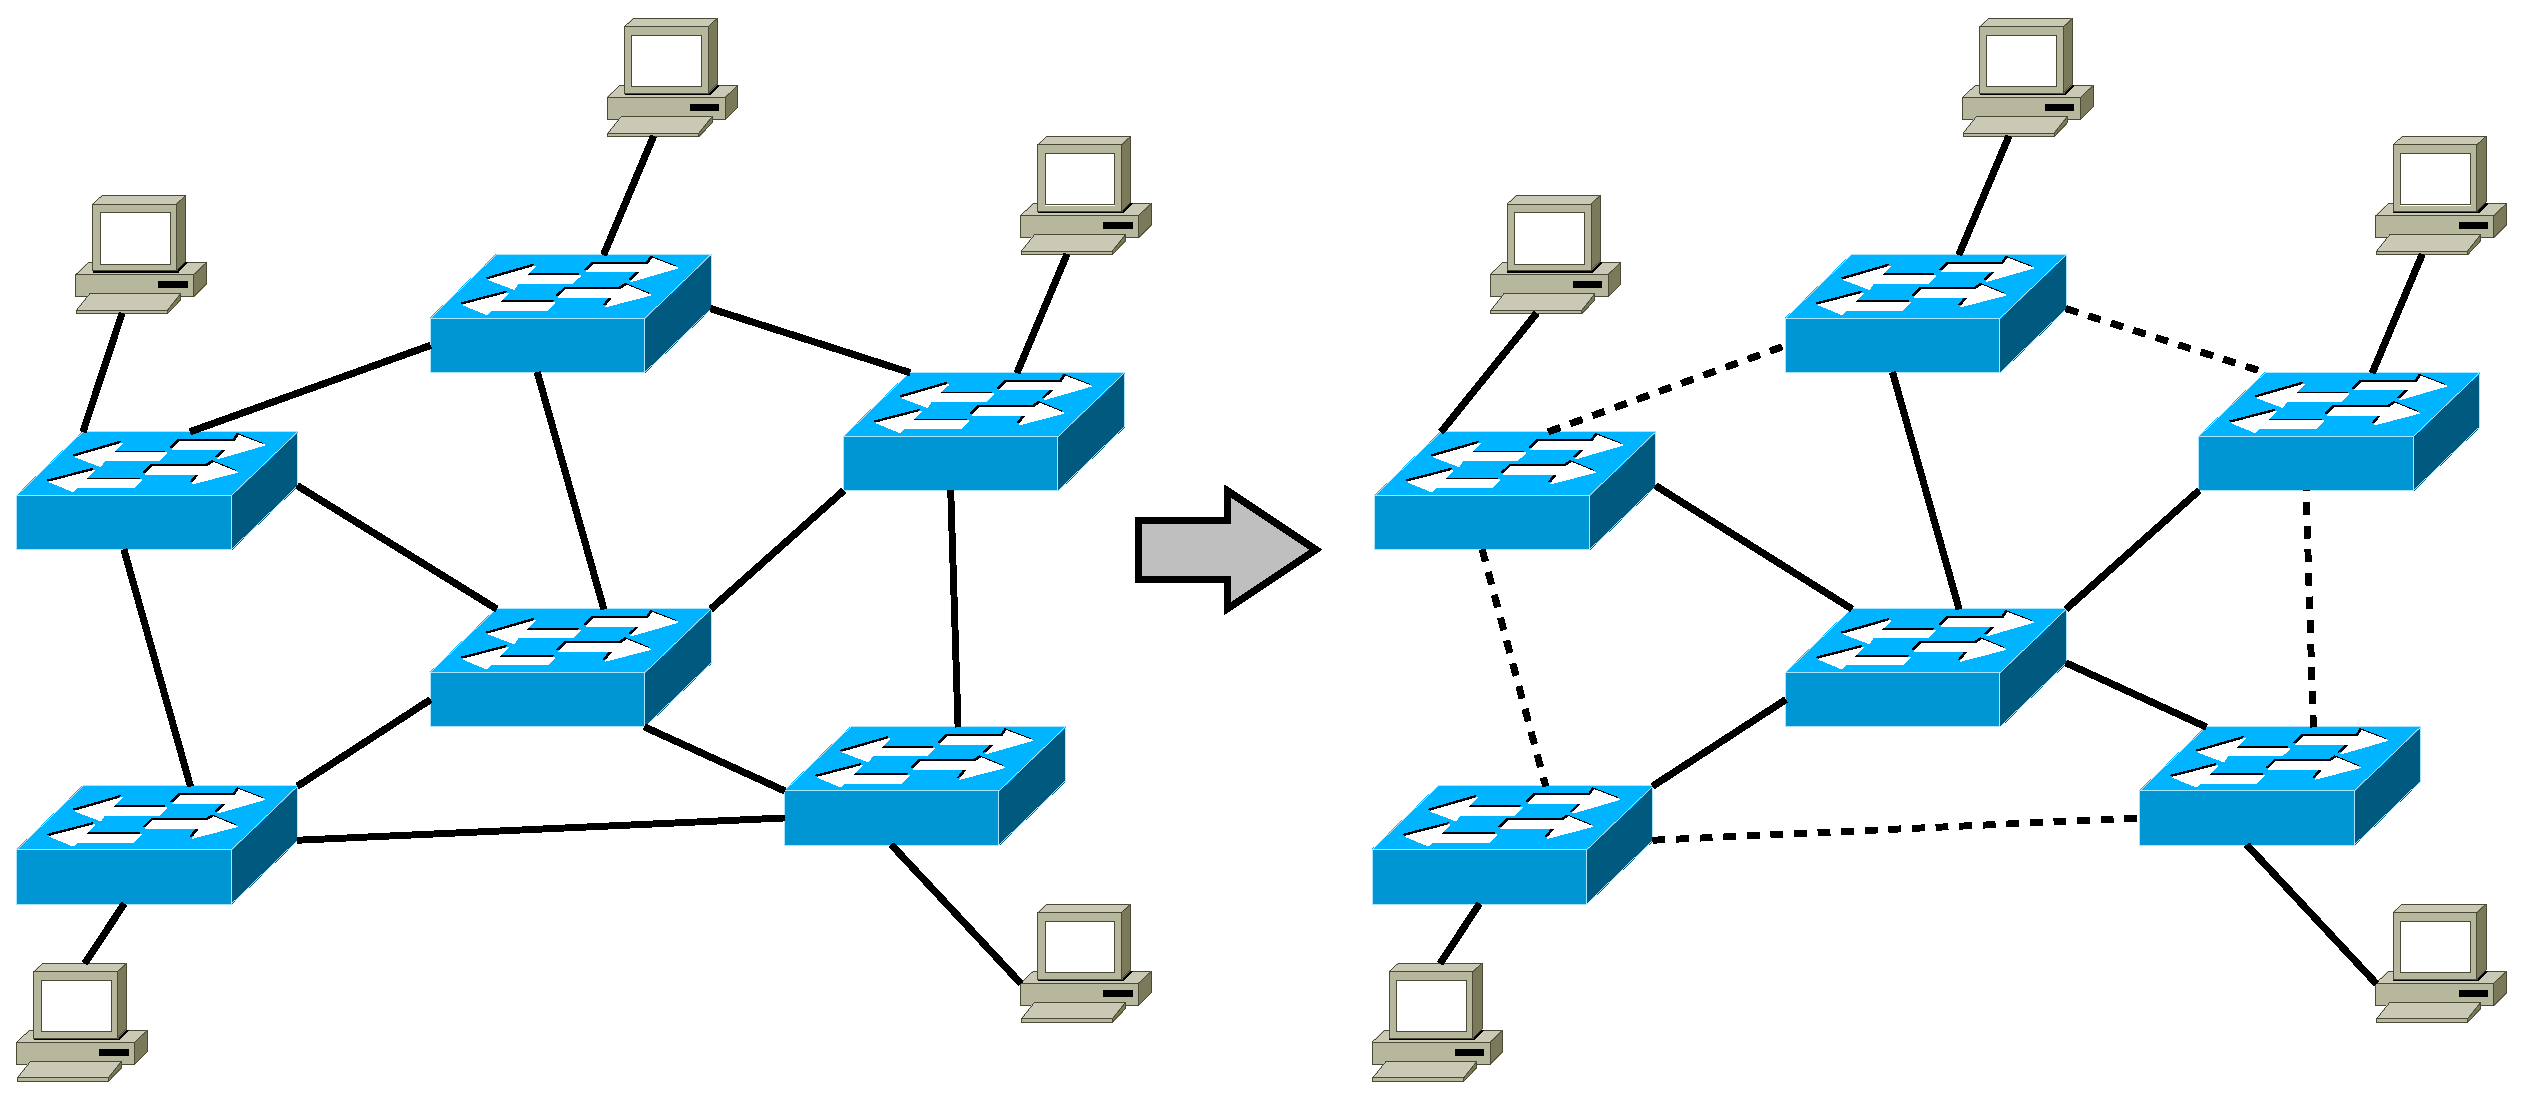
\includegraphics[width=\linewidth]{figures/stp.eps}
 \caption{Protecting ethernet segments from loops with \gls{stp}}
\label{fig:stp1}
\end{figure}
This situation is shown in Figure \ref{fig:stp1}: on the left side, the physical connections are shown, containing loops. 
\gls{stp} removes
the loops by setting certain interfaces to blocking mode, connected by dotted lines, as shown on the right side of Figure \ref{fig:stp1}.
\\
The algorithm works as follows:

\begin{itemize}
 \item The first step of the \gls{stp} algorithm is to nominate one device as root bridge\footnote{the terms \textit{switch} and \textit{bridge} are used synonymously,
with the major difference that switches can break network segments into multiple subsegments through \glspl{vlan}}. This can be done manually by the network administrator,
or dynamically through the exchange of packages containing a priority. All switches will agree on lowest priority device as root bridge, additionally using the unique
hardware \gls{mac} address if collisions occur. The root bridge sets all interfaces to forwarding mode. 
 \item Afterwards, every switch determines the path with minimal costs for reaching the root bridge. The cost of every connection can be determined by the link
 speed or configured by the network administrator manually
 \item Finally, all devices except the root bridge set the ports belonging to the minimal-cost path to forward mode. All other ports are set to blocking mode, thus removing
 any loops.
\end{itemize}
If a connection is lost and an ethernet segment is not 
reachable any more, the \gls{stp}, although not primarily designed for that tasks, can be used to handle that fault. Nodes affected by the link-change report
that event to the root bridge, so that the network can be re-configured and a different path can be established, thus re-connecting the unreachable segment
and providing fault tolerance. 
\\
\\
A big drawback of this mechanism is the topology-dependent
time needed for network re-organization. While in simulations delays of millisecond magnitude can be achieved \cite{4447112}, in practice link recovery
can take up to one minute which is not acceptable for many industrial environments. An improvement was achieved with \gls{ieee} 802.1w \gls{rstp} and
a variety of different proprietary protocols, not compatible to each other, but still no sufficient recovery times were achieved \cite{1704183}.

\subsubsection{IEC 62439}

As it turned out that the mechanisms based on \gls{stp} and its variations were not 
sufficient for many applications, the family of IEC 62439 standards was defined. IEC 62439 introduces a set of ethernet extensions, assuring high availability
and enabling its deployment in industrial applications. Three extensions are introduced below.

\subsubsection{\gls{mrp}}
After IEC 62439-1 specifying basic definitions, the second draft introduced \gls{mrp} which confines network outages to less than 500ms \cite{6145654}.
This is achieved by restricting the valid topologies to ring-only, so all switches are connected to the network by 2 interfaces. All switches beside the ring manager
forward all traffic received, while the ring manager opens the loop logically by setting one of its interfaces to blocking mode.
In this mode, all packages except management messages are discarded. The ring manager detects a failure by periodically sending test management messages in both
directions. Additionally every node is able to detect a link failure on its local ports. It then sets the port to blocking and signals this link failure to the
ring manager which opens his second port by setting it to forward mode and therefore reconnects the unreachable segment.
\\
\gls{mrp} does not rule out package loss in case of a failure, therefore it can be seen as improved \gls{rstp} for ring topologies. 

\begin{figure}[H]
 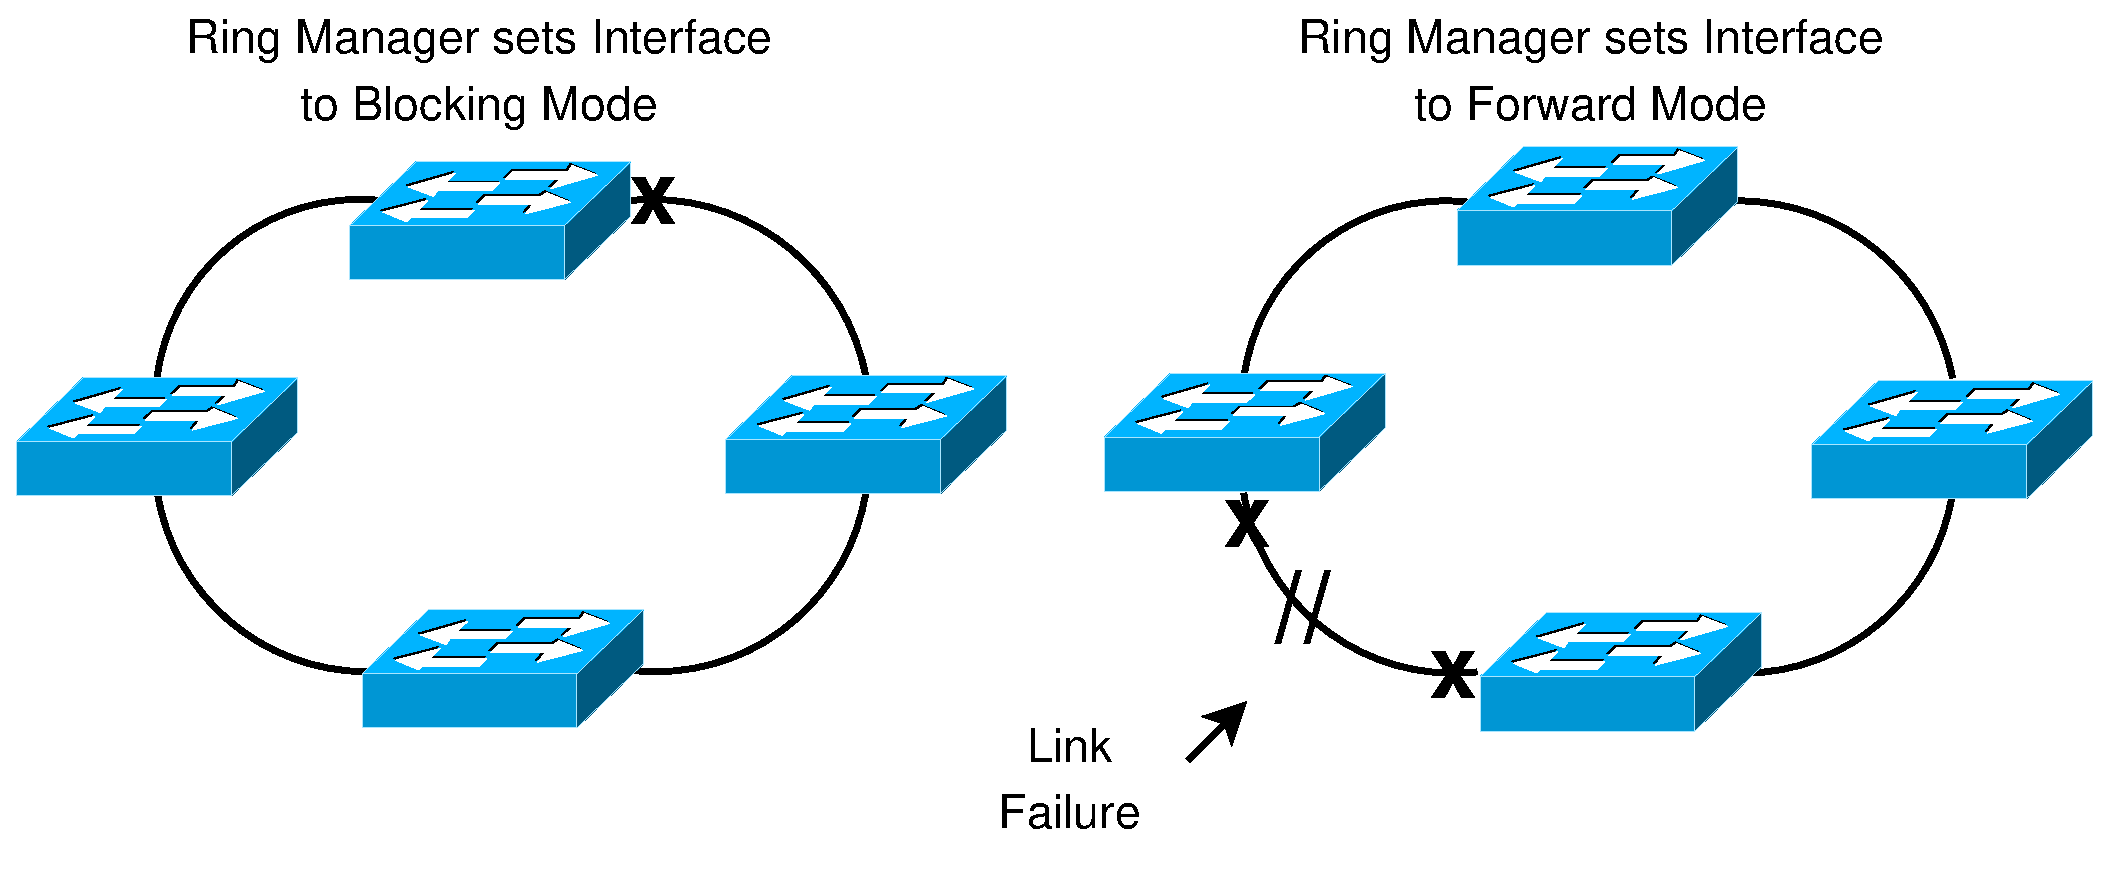
\includegraphics[width=\linewidth]{figures/MRP2.eps}
 \caption{MRP fault tolerance}
\label{fig:mrp1}
\end{figure}


\subsubsection{\gls{prp}}
In 2010, IEC 62439-3 defined a first version of {\gls{prp}} and \gls{hsr}, both suitable for hard real-time
systems \footnote{hard real-time characterizes a system where missing of a dead line may result in a catastrophic event} \cite{4416946}.
\\
In 2012, IEC 62439-3 was revised, defining new versions of \gls{prp} and \gls{hsr}. The basic ideas behind both protocols remained
unchanged, so the latest versions are described below.
\\
\\
\gls{prp} can tolerate a link fault without package loss by utilizing two redundant and independent \glspl{lan}.
Nodes needing high availability, called \gls{danp}, are connected to both networks by two interfaces, sharing the same \gls{mac} and \gls{ip} addresses.
Additionally, standard ethernet devices called \gls{san} can be connected to only one network, enabling communication with devices on the same \gls{lan} only.
An example of such a network is shown in Figure \ref{fig:prp}.
\\
To support redundant connections for \glspl{danp}, a sub-layer on \gls{osi}-layer 2 (i.e. the link layer), called \gls{lre} is defined. 
Upper level data arriving at the \gls{lre} of a \gls{danp} is duplicated and equipped with 6 bytes of control information, containing a 2 byte sequence number,
\gls{lan} number, length information and a static suffix identifying the \gls{lsdu} as \gls{prp} traffic. The sequence number is used for duplicate detection: 
every node uses one global counter $Ctr_{global}$ for outgoing messages, not discriminating the receiver. For every package sent, the sequence number is incremented.
Additionally, every node maintains distinct counter values $Ctr_{source}$ for every unicast source-address it receives messages from, as well as for multicast
and broadcast messages.
\\
On the receiving side the \gls{prp} traffic is detected because of the suffix, duplicates can be discarded by utilizing the sequence number \cite{6699852}.
The standard does not dictate how this must be achieved, it only demands that legitimate packages must not be discarded. Because of the short global outgoing 
sequence number, duplicates may not be detected as such - responsibility for final detection is delegated to upper layers.
%If the received number is higher than the saved one $C_{source}$, the package is forwarded to the upper layer and the received sequence number is saved as $C_{source}$.
%Therefor, the package transmitted over the alternate line (i.e. the delayed package) will contain a sequence number smaller than the number saved for the 
%corresponding source address and can safely be discarded, thus preventing the processing of duplicate frames by the upper level.  
\begin{figure}
    \centering
    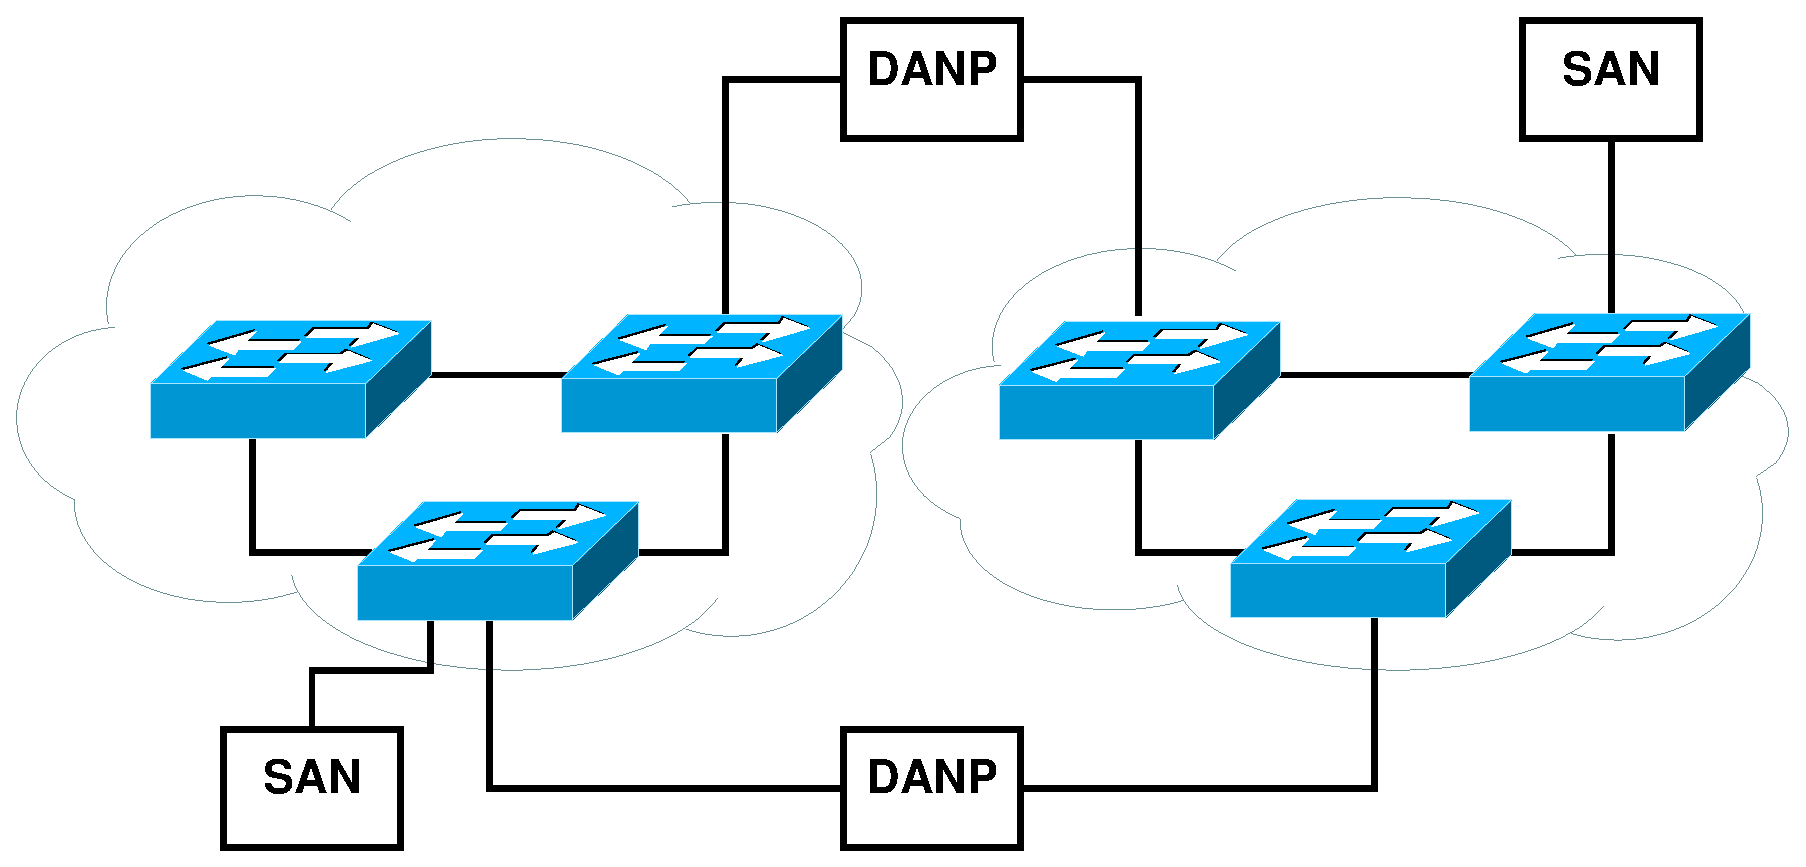
\includegraphics[width=1\textwidth]{figures/prp.eps}
    \caption{\gls{prp} network}
    \label{fig:prp}
\end{figure}

\subsubsection{\gls{hsr}}
\gls{hsr} is based on ring-topology, but it also allows to connect \gls{hsr} and \gls{prp} networks, different \gls{hsr} rings or even to build a ring of rings. 
Every node is connected to the network by two interfaces, duplicating data from upper layers and sending one copy in clockwise, the other copy in counter-clockwise direction,
thus eliminating the need for duplicated networks but wasting about half of the available bandwidth \cite{6174793}. 
\\



%%%%%%%%%%%%%%%%%%%%%%%%%%%%%%%%%%%%%%%%%

%%%%%%%%%%%%%%%%%%%%%%%%%%%%%%%%%%%%%%%%%
\chapter{KNX}
\label{ch:knx}
\input{chapters/knxGeneral}
\input{chapters/knxLayers}
%\section{Security in HBAS}\label{hbaSec}
\glspl{hbas} emerged from automation systems, originally used for building control, summarized as \gls{hvac}.
Central building management, leading to \textit{intelligent buildings}, promises
reduced maintenance costs, energy savings and improved user comfort \cite{1435745}, compensating the initially higher investment costs of such buildings.
Following these arguments it would be natural to integrate additional building management functions like alarm systems, access control or communication systems,
exploiting already existing infrastructure like cabling and thus benefiting from synergy effects.
\\
This trend was contradicted by the fact that in the early days of \gls{hbas}, communication security was not considered a critical requirement.
Firstly, the communication was done over wires,
i.e. physical access to the network would have been necessary for attacking the network \cite{knxSpec}. Secondly, the possible threats by misusing \gls{hvac} applications
were considered negligible. Additionally, the devices used in such networks were characterized by very limited processing power - thus, the comprehensive
use of cryptographic measurements would have put remarkable computing loads onto these devices and was therefore considered impracticable.
\\
These arguments turn out to be true only at first glance. Because \gls{hbas} are operational over years, excluding short-time, temporary physical access is often impossible
for wired networks and nearly impossible for
wireless networks. Regarding the second argument it is easy to see that simple acts of vandalism, for example shutting down the lighting system of a company building, can result
in considerable financial losses.
\\
\\
Today the necessary processing power is available even on embedded systems, meanwhile systems integration continued until a point where security concerns could
no longer be neglected. It follows that such a \gls{hbas} must be protected against misuse on all existing levels. 
Communication networks for \gls{hbas} systems are usually built upon a two-tier model, consisting of a field- an a backbone level. The field level contains \glspl{sac},
interacting with the environment and performing the control functions. They are interconnected by the backbone network. Here, \glspl{md}, used for configuration,
visualization and monitoring, as well as \glspl{icd}, connecting physical segments, are found. Special \glspl{icd} may act as gateways, providing a connection to foreign networks. 
\\
\\
Due to this topology, two different classes of attacks are possible: network- and device attacks \cite{5332331}.

\subsubsection{Network attacks}
Here, the adversary either tries to compromise the field or backbone network. In the first scenario, the attacker can analyze or modify the control application. In the latter he
gains access to the concentrated network data and can thus obtain a global view of the system.
\\
To protect a communication network it would be possible to use security mechanism known from the \gls{ip} world. 
Unfortunately, these mechanisms often cannot be mapped directly to \glspl{hbas} because of the introduced overhead. Using
established techniques like \gls{vpn}, \gls{tls} or \gls{ipsec} is therefore reserved for the backbone level where \gls{ip} is used.
\\
At the field level \gls{ip} is hardly ever used, a fact that excludes \gls{ip} based technologies here.

\subsubsection{Device attacks}
Alternatively, the three different kinds of devices can be aimed at by either attacking a \gls{sac} to manipulate it's behavior or by attacking a \gls{icd} to access data of the segment.
Finally, the attacker can launch an attack against the \glspl{md} to gain management access to the other two types of devices.
\\
Such device attacks are divided into three categories: software attacks, side-channel and physical attacks, extensively surveyed in \cite{5332331} and \cite{secAn}.	% moved content to chap 1 / problem statement
\section{KNX security concept}
As shown in section \ref{hbaSec}, a paradigm shift towards towards increased security in \gls{hbas} can be observed. 
Despite that fact, the basic \gls{knx} standard does not specify any security mechanisms for control information:
\\

\textit{"For KNX, security is a minor concern, as any breach of security requires local access to the network. 
In the case of KNX TP1 or KNX PL110 networks this requires even physical access to the network wires,
which in nearly all cases is impossible as the wires are inside a building or buried underground.
Hence, security aspects are less of a concern for KNX field level media."} \cite{knxSpec}
\\
\\
For \gls{knx}/\gls{ip}, the physical containment arguments do not apply. To counter this, it is proposed to use firewalls and \glspl{vpn} to prevent unauthorized access,
as well as hiding critical network parameters from public. The latter concept is also known as \textit{"security by obscurity"}, offering - if at all - only 
little protection.
\\
For management communication, a rudimentary, password-based control is used. Therefore, \gls{knx} suffers the following security flaws 
\cite{Granzer05securityin}: for management, the 
used keys are transmitted as cleartext, enabling an attacker to perform a passive attack to obtain the password. Subsequently, the attacker can mount an active
attack, injecting
arbitrary management messages. No methods are foreseen for generation or distribution of the keys.
For control information, an adversary can directly inject arbitrary messages to control the network, allowing passive and active attacks too.
These shortcomings clearly disqualified \gls{knx} for usage in critical environments, restricting its possible field of application.
\\
Today, \gls{hbas} systems are used on a large scale, and the available processing power on embedded computing platforms has risen significantly, so the deployment
of such systems would be possible also in critical environments, under the condition that proper security mechanisms are deployed. For \gls{knx}, several extensions
exist which will be introduced in the next sections.

\subsection{KNX Data Security}

In 2013, the KNX association published "Application Note 158" \cite{knx_data_sec} which specifies the \gls{knx} \gls{s-al}, providing
authentication and encryption, and the \gls{ail}, implementing access control, booth being part of the application layer.
The settlement of these functions above the transport layer allows a transparent, communication media independent end-to-end encryption.
\\
The application layer service code 0xF31 is reserved for this purpose, indicating that a secure header and a \gls{s-al} \gls{pdu} 
follow instead of a plaintext-\gls{pdu}. This allows the flexible usage of the secure services just in situations where they are needed - otherwise, the plaintext application
layer services can be used.
\\
The \gls{s-al} services defines modes for authenticated encryption or authentication-only of a higher-level cleartext \gls{apdu}. As underlying block cipher
\gls{aes}128 is used in \gls{ccm} mode, encrypting the payload with \gls{ctr} and providing integrity with \gls{cbc} mode. The overhead introduced by the 
\gls{mac2} is reduced by 
using only the 32 most significant bits instead of the whole 128 bit block obtained from \gls{cbc}. Source- and destination address as well as
frame- and addresstype, the \gls{tpci}, length information and a 6 byte sequence number determine the \gls{iv} for the \gls{cbc} algorithm and are therefor also protected by the \gls{mac2}.
The sequence number is a simple counter value that provides data freshness, thus preventing replay attacks, and is sent along with every \gls{s-al} \gls{pdu}.
For synchronization of this sequence number between two devices, a \gls{s-al} s	ync-service is defined. Because no sequence number can be used here to guarantee
data freshness, a challenge-response mechanism is used instead.
Two different types of keys are used: a \gls{fdsk} is used for initial setup with the \gls{ets}. The \gls{ets} then generates the \gls{tk}, which is used by the
device for securing of the outgoing messages. Consequently, every device must know the \gls{tk} of it's communication partners.
\\
\\
While the \gls{s-al} empowers two devices to communicate in a secure way, the \gls{ail} allows a fine-grained control which sender has access to which
data objects. Therefore, every \textit{link} (a combination of source address and data or service object) is connected with a \textit{role}, which in turn
has some specific \textit{permissions}. 

\subsection{EIBsec}

EIBsec is another extension to \gls{knx}, providing data integrity, confidentiality and freshness, allowing its deployment in security-critical environments.
A semi-centralized approach is taken here by using special key servers, responsible for dedicated sets
of keys, providing a sophisticated key management. EIBsec divides a \gls{knx} network into subnets, connected by devices called \gls{acu}. Beside their native
task, i.e. routing traffic, they
 are responsible for the key management of their network segments, which includes key generation, distribution and revocation. Every standard device that
 wishes to communicate with other devices must at first retrieve the corresponding secret key from its responsible \gls{acu}, which can therefor control the
 group membership of the requesting device by allowing or denying the request respectively by revoking the key at a later point in time.
\\
EIBsec uses two different keys: in normal mode, a session with the keyserver is established to retrieve the session key, establishing a secure channel.
This mode uses encryption-only by utilizing a \gls{psk}, integrity must therefor be guaranteed by the sender of the message. Counter mode is used for transmitting management and
group data over the secure channel. A simple \gls{crc} is added to the payload before encryption and shall guarantee integrity. Booth modes encrypt the traffic
on transport level, allowing standard routers to handle the datagrams. As block cipher, \gls{aes}-128 is used in \gls{ctr} mode.

\subsection{KNX IP Security}

This work focuses on securing the \gls{knx} \gls{ip} specification, which can be used as backbone for connecting distinct \gls{knx} installations \cite{5195839}.
Thanks to the widespread use of \gls{tcp}/\gls{ip}, a wide range of physical transport mechanisms can be utilized.
\\
A structure comparable to the design of \gls{tls} is defined by building a distinct security layer, residing above the transport layer (therefore, it directly
connects the transport to the application layer, because session- and presentation layer are empty, as defined by the \gls{knx} specifications, see chapter
\ref{ch:knx}).
\\
The design distinguishes 3 different types of modes: 

\begin{itemize}
 \item In the \textit{configuration phase}, every device that wants to participate in the secure network
generates an asymmetric key pair, which is sent to the \gls{ets} over a secure channel (for example, by transmitting the data over a direct, serial connection
between the \gls{ets} host and the \gls{knx} device).
The \gls{ets}, acting as \gls{ca1}, signs the combination of \gls{ip} and public key with its own private key, thus generating a certificate, which is sent back to the device, along
with the public key of the \gls{ets}. 
 \item After that, the \textit{key set distribution phase} starts, where a unicast and a multicast scenario are differentiated:
in the unicast case, the device initiating the communication - called client - obtains the key set from the target device by a 2-step handshake: at first, mutual entity 
authenticity is established by utilizing the certificate provided by the \gls{ets}. Afterwards the keyset is obtained from the target, which concludes the second
phase.
\item In the last step, secure communication can take place, i.e. the the client is able to
encrypt the data with the obtained key and sends it to the target device.
\end{itemize}
For the multicast scenario, a distinct \textit{coordinator}, responsible for maintaining the group key, is necessary. Every powered-up device
identifies the coordinator as soon as possible by broadcasting \textit{hello} requests, adopting the coordinator role if no replies are received in time.
To actually send a payload, the group key is obtained from the coordinator and the data is sent to the group, analog to the unicast case.
By adding mechanisms to detect "dead" coordinators and delegating the coordinator role to a different device, the design avoids a \gls{spof}.


\section{Summary}
Examining the security measurements shows up parallels to the \gls{ipv4} world. As with \gls{knx}, no security measurements were foreseen in the
original standard. The problem was
fixed here in two ways: \gls{tls} was added as a sublayer between \gls{osi} layers 4 and 5, allowing application-transparent encryption and authentication, 
similar to KNX Application Note 158, as described above. The second solution was the introduction of \gls{ipsec}, extending \gls{ipv4} and thus enabling authentication and encryption on \gls{ip} level.
\\
\\
Despite the \gls{knx} extensions, no solution providing high availability exists. Therefore, this work proposes a to combination of cryptographic measurements with
redundancy mechanisms, allowing its deployment in more demanding environments.

%%%%%%%%%%%%%%%%%%%%%%%%%%%%%%%%%%%%%%%%%

%%%%%%%%%%%%%%%%%%%%%%%%%%%%%%%%%%%%%%%%%
\chapter{Concept}
\label{ch:concept}
\input{chapters/securityconcept}

%%%%%%%%%%%%%%%%%%%%%%%%%%%%%%%%%%%%%%%%%

%%%%%%%%%%%%%%%%%%%%%%%%%%%%%%%%%%%%%%%%%
\chapter{Evaluation}
\label{ch:implementation}
\label{chap5}
\section{Master daemon}

\subsection{KNX addressing scheme}

Care must be taken that no duplicate \gls{knx} addresses are used within the network. Therefore, the following addressing convention is proposed:
While it would be possible to use the same addresses on both lines per gateway, a different scheme is used.
For the secured network, the address ranges starting at address 1.1.1 to address 1.1.15 and 1.2.1 to 1.2.15 are reserved for secure line number
1 and 2 respectively, which allows a maximum of 15 gateways. Different addresses are used mainly because it facilitates debugging. 
On the unsecured lines, every gateway uses an address from the range 1.0.1 - 1.0.15. Addresses are assigned in a linearly ascending way, so gateway number 1
uses addresses 1.1.1 and 1.2.1 for secure lines 1 and 2, and 1.0.1 for its unsecured line.

\section{Evaluation}

\subsection{Synchronization phase}
Packages in the synchronization phase are not encrypted, allowing a passive adversary to learn the value of the global counter value $Ctr_{global}$. Nevertheless,
this counter is only used to avoid deterministic encryption (see \ref{deterministicEnc}) and is of no use for the attacker.
\\
\\
Opening a window for tolerating timing deviations allows an active attacker to inject a captured synchronization response package within that time window.
Nevertheless, because the header is protected by a \gls{mac2}, the only way to inject a synchronization package is to use exactly the same frame as captured,
i.e. the same source address, which will be discarded because the the requesting device already finished the synchronization stage.
\\
Additionally, the counter value is of no use for the attacker, as described above.

\subsection{Discovery phase}

\subsection{Data transmission phase}


\subsection{High Level Cryptography Library}

\subsubsection{OpenSSL}

\begin{itemize}
 \item install libssl, libssl-dev
\end{itemize}



%%%%%%%%%%%%%%%%%%%%%%%%%%%%%%%%%%%%%%%%%

%%%%%%%%%%%%%%%%%%%%%%%%%%%%%%%%%%%%%%%%%
\chapter{Results}
\label{ch:conclusion}
\section{Contribution}
To be able to deploy a communication system in more demanding environments, it is necessary to achieve informational security combined with mechanisms for improved availability.
For \gls{knx}, extensions for securing a network against malicious attacks exist, but these extension are not able to handle a fault concerning the communication medium, as well
as \gls{dos} attacks.
Therefore, this work proposes a way to protect against transient hardware failures, as well as active and passive adversaries. For the latter, the proposal is able to resist
restricted \gls{dos} attacks, too. This is achieved by using security gateways which are connected to each other in a redundant way. Standard \gls{knx} devices are connected 
through these gateways, which copy the client's frames into two properly secured frames and send them over both communication lines. The receiving side will check the received
frames for modification, discard one of the two copies and forward the remaining one to the destined standard \gls{knx} device.
\\
\\
It was shown that the proposed solution can withstand malicious attacks, as well as transient hardware failures of one of the secured lines. Therefore, the solution allows to connect
standard \gls{knx} devices which are spatially divided in a secure manner, bridging over areas where malicious behavior cannot be ruled out.
The proposed solution can be deployed in a 'plug-and-play' 
manner, as long as the constraints defined in Section \ref{sec:opContraints} are regarded. Thus, it is possible to add confidentiality, integrity and availability to a \gls{knx}
network just where needed, coexisting with segments with low security demands. By using more than 2 secured lines, the solution can easily be extended to use $n$ instead of 2 secure threads
and communication lines, increasing availability to an even higher level.

\section{Outlook}

The following improvements to the prototype solution are proposed: 
\begin{itemize}
 \item Using a cache for the mapping of group address to security gateways and encryption keys. A gateway receiving data from a client would send a discovery message once and
 cache the address(es) of the responsible gateway(s), together with the corresponding encryption key(s). Subsequent data transfer can be executed without the need for sending
 discovery messages first, reducing the bus load. Of course, a reasonable caching time has to be found after which a cached entry is deleted because newly connected
 clients may not be reachable within this duration.
 \item Obfuscating the size of the data service messages, which  can be achieved by adding an additional length field and corresponding padding, chosen randomly. This makes it harder
 to derive communication profiles.
 \item Attacks can be detected if frames with forged \glspl{mac2} are received, allowing to send an alert to an operator. For the used platform, this can be achieved easily by connecting
 the RaspberryPis to a restricted \gls{ip} network and sending the alarm, for example, by mail or \gls{snmp}.
 Additionally, the address of the attacking device can be added to a blacklist such that traffic coming from this address is discarded immediately.
 \end{itemize}
 
\subsubsection{Restrictions }
During development, the follow restrictions were found. Of course, the constraining assumptions made in Section \ref{sec:opContraints} are still valid. 

\begin{itemize}
  \item While \gls{eibd} can send extended frames, it does not support receiving frames with payload $\geq$ 56 byte. While this clearly violates the \gls{knx} specification, no efforts
  were made to debug this behavior.
  \item With the current \gls{eibd} \gls{api}, sending raw frames is not possible, but only application- or transport layer data units. This implies that 
  it is not possible to set the source address of a written frame. Frames delivered by a security gateway are therefore sent with the gateway's device address, instead of the 
  origin device address. To make the security gateways appear fully transparent to client devices, the \gls{api} must be extended.
 \end{itemize}


 
 

%%%%%%%%%%%%%%%%%%%%%%%%%%%%%%%%%%%%%%%%%


\appendix

%%%%%%%%%%%%%%%%%%%%%%%%%%%%%%%%%%%%%%%%%
\nocite{*}	% generate complete bibliography without corresponding \cites{}

%%%%%%%%%%%%%%%%%%%%%%%%%%%%%%%%%%%%%%%%%
\chapter{Setup of the base system}
\label{ch:basesystem}
\input{chapters/app.tex}
%%%%%%%%%%%%%%%%%%%%%%%%%%%%%%%%%%

\printglossary
\printbibliography

\end{document}
